\documentclass[11pt,a4paper]{article}
\usepackage[T1]{fontenc}
\usepackage{lmodern,amsmath,amssymb,amsthm,mathtools,booktabs,graphicx,microtype,array}
\usepackage[margin=25mm]{geometry}
\usepackage{xcolor,fancyhdr,needspace,pdfpages}
\usepackage[colorlinks=true,linkcolor=blue!45!black,urlcolor=blue!50!black]{hyperref}
\pagestyle{fancy}\fancyhf{}\lhead{Joint resources for causal quantum recovery}\rhead{5 November 2026}\cfoot{\thepage}
\setlength{\headheight}{14pt}\setlength{\parindent}{0pt}\setlength{\parskip}{6pt}
\newtheorem{theorem}{Theorem}\newtheorem{corollary}{Corollary}\newtheorem{lemma}{Lemma}
\newcommand{\id}{\operatorname{id}}\newcommand{\Tr}{\operatorname{Tr}}\newcommand{\SWAP}{\operatorname{SWAP}}
\newcommand{\dd}{d_\diamond}\newcommand{\norm}[1]{\left\lVert#1\right\rVert}
\newcommand{\Acal}{\mathcal A}\newcommand{\Ncal}{\mathcal N}\newcommand{\Ecal}{\mathcal E}
\title{\vspace{-1em}The joint resource question for causal recovery\\from a homogeneous tracial partial-SWAP stream\\[.5em]\large Exact acquisition accounting, physical processing obstructions,\\and the remaining optimal-memory problem}
\author{Astra research continuation and reproducibility record}
\date{5 November 2026}
\begin{document}
\maketitle
\begin{abstract}
The full optimal memory/processing law is not resolved in this continuation.
The preserved all-prefix crossing converse, positive general-instrument witness,
and exact pre-access loss law remain valid. A changing-reference Hilbert-space
representation now gives a nonnegative, exact acquisition-loss ledger for every
permitted causal CPTP receiver, including nontracial initialized workspace and
unlimited classical feedback. Its final value determines an attained Petz-twirled
recovery error and an all-decoder lower bound within a factor two. Consequences
include a quantum retention-duration bound, a joint finite-count strengthening of
the crossing converse, and a dimension-independent error floor for uniformly weak
carrier-dependent readers that discard spent carriers. A Yangian Dirichlet form
identifies fixed-prefix fourth-order leakage, with a rank-sensitive spin-sector
constraint. A positive three-carrier instrument has an exact physical decoder
and a paid packed-memory rate approaching 0.730 qubits per carrier, but has a
nonzero accuracy floor. A new smooth energy-window instrument instead gives
arbitrary-accuracy physical compression with exact angle/count bounds, actual
support embeddings and a reverse decoder. An elementary version proves a strict
weak-angle memory-coefficient improvement over the full-storage inverse reader,
after paying extra acquisition and circuit service; its generic block processing
is exponential and its retained width still has quartic angle scaling.
Initialized coherent frames expose a distinct slow dynamics and an all-width
phase-reference converse, with an explicit finite-angle lift. An exact polynomial
certificate identifies why scalar normalization of the existing crossing argument
cannot close its logarithmic gap. Exact finite-policy optimization is attainable
in principle but has not been
evaluated into the requested scaling. All limits and remaining construction
gaps are stated explicitly.
\end{abstract}

\section{One endpoint, unchanged physical premises}
An unknown qubit $S$, possibly entangled with an inaccessible reference $R$, meets
independent carriers $E_j$ in $\tau=I/2$. Every source encounter is
\[
 U_j=cI+is\SWAP_{S,E_j},\qquad c=\cos\theta,\ s=\sin\theta,\quad0<\theta<\pi/2.
\]
The receiver accesses outputs once, chronologically; the final source is
discarded. Arbitrary initialized workspace, CPTP instruments, classical histories
and feedback are allowed. Every coherent buffer counts. No bath purifier,
preparation key, return link or changed emitter is supplied. Error is half
diamond distance from the identity channel.

The endpoint is the attainable joint relation among $\theta,\epsilon,N$, peak
coherent storage and processing, with preparation, service, protection and
finite control accounted for. A restricted-reader obstruction, a fixed-angle
asymptotic, or an implicit optimum definition is not this full endpoint.

The earlier Astra acquisition calculation and completed peer spectral-profile
converse are inputs [A1,A2]. Their preserved extension [A3] is included as an
unchanged proof-note appendix and a separate original file in the archive.
It contains the crossing proof, refined positive-instrument witness, exact
carrier-loss law and physical reverse decoder, with their prior attribution.

Put $b=s^4$, $r=1-b$, $\ell=-\log r$. Storing all $N$ outputs and applying
inverse collisions to an independent mixed dummy in reverse chronology gives
\begin{align}
 \mathcal D_N\mathcal C_N&=(1-r^N)\id+r^N\mathcal R_{I/2},
 &\epsilon_P&=\tfrac34r^N,\\
 \epsilon_{\rm opt}&\ge\tfrac34(1-\sqrt{1-r^N}).
\end{align}
Thus $N=\Theta(\theta^{-4}\log(1/\epsilon))$ jointly at weak angle and high
accuracy. Source forgetting has visibility $c^{2N}$ and a quadratic clock.
At each fixed nonzero angle the preserved general bound is
\[
 q_{\rm peak}=\Omega_\theta\!\left(\frac{\log(1/\epsilon)}
 {\log\log(1/\epsilon)}\right)=\Omega_\theta(N/\log N)
\]
at the benchmark, versus the known $O(N)$ upper bound. The logarithmic gap and
the weak-angle fixed-error optimum remain open here.

\section{An exact positive ledger for every causal receiver}

Let $\Ncal_j:L\to SM_j$ be the channel after update $j$, where $L$ is the initial
logical qubit. Include all classical histories in $M_j$ as a direct sum, and all
initialized quantum workspace. The exact invariant is
\begin{equation}
 \Ncal_j(\tau)=\tau_S\otimes\sigma_j.\label{eq:baseline}
\end{equation}
For tracial logical input, each fresh $SE_j$ pair is tracial and independent of
the receiver before its collision. The source unitary leaves this average
unchanged; the receiver then acts only on $M_{j-1}E_j$. This proves the product
form inductively, including conditional classical blocks. It asserts no such
independence for nontracial input or for the Bell state with its reference.

For the three Pauli directions define balanced operators
\[
 X_{\mu,j}=(\tau_S\otimes\sigma_j)^{-1/4}\Ncal_j(\sigma_\mu/2)
 (\tau_S\otimes\sigma_j)^{-1/4}.
\]
All inverses are on support; positivity puts the logical images on that
support. Use ordinary Hilbert--Schmidt norms, summing classical blocks. Let
$P(X)=I_S\otimes\Tr_S(X)/2$, $Q=I-P$, and
\[
 a_j=\frac13\sum_\mu\norm{PX_{\mu,j}}_2^2,\qquad
 q_j=\frac13\sum_\mu\norm{QX_{\mu,j}}_2^2.
\]
Here $q_j$ is an information norm, not a qubit count. Initially $a_0=0,q_0=1$
for any independent receiver initialization.

\begin{theorem}[All-receiver acquisition ledger]
Every permitted causal receiver has nonnegative losses $\ell_j^P,\ell_j^Q$
with the exact relations
\begin{align}
 a_j&=a_{j-1}+bq_{j-1}-\ell_j^P,&q_j&=rq_{j-1}-\ell_j^Q,\\
 a_j+q_j&=1-\sum_{k\le j}(\ell_k^P+\ell_k^Q),\nonumber\\
 a_N&=1-r^N-L_N,&
 L_N&=\sum_{j=1}^N[\ell_j^P+(1-r^{N-j})\ell_j^Q].\label{eq:ledger}
\end{align}
The actual memory channel $\Ecal_N=\Tr_S\Ncal_N$ has Petz entanglement
fidelity $(1+3a_N)/4$. Every final decoder obeys
\begin{equation}
 \epsilon_{\rm opt}\ge\tfrac34(1-\sqrt{a_N}).\label{eq:lowera}
\end{equation}
A finite global Clifford twirl of the receiver and its physical Petz decoder
attain
\begin{equation}
 \epsilon_{P,\rm twirl}=\tfrac34(1-a_N)=\tfrac34(r^N+L_N).\label{eq:attained}
\end{equation}
Petz is CPTP here; cheap synthesis and fast service are not assumed.
\end{theorem}

\begin{proof}
For a CPTP map $\Lambda$ taking average $\omega$ to $\sigma$, the relative map
\[
 V(X)=\sigma^{-1/4}\Lambda(\omega^{1/4}X\omega^{1/4})\sigma^{-1/4}
\]
is a Hilbert--Schmidt contraction. This is the monotone quantum $\chi^2$ metric
with $f(t)=\sqrt t$ [1], or follows by expanding sandwiched R\'enyi-2 data
processing [2,3] at $\omega+tA$. Trace preservation cancels the constant and
linear terms. A trace normalization, when needed, cancels on both sides.
Hermitian and anti-Hermitian parts give the general contraction. Continuous
classical outcomes are handled by direct integrals in place of direct sums.
On $SME$ it acts as $\id_S\otimes V$, preserving and contracting $P,Q$
separately, including all classical direct sums.

Appending $\tau_E$ appends $I_E/\sqrt2$ in balanced coordinates. The source
unitary commutes with the average and therefore acts unitarily. The accepted
collision orthogonality [A1] gives
$a_j^-=a_{j-1}+s^4q_{j-1}$ and $q_j^-=rq_{j-1}$. Newly exported
source-identity terms have a traceless fresh-carrier factor and are orthogonal
to old exports. All old receiver coefficients remain in this identity. Set
$\ell_j^P=a_j^--a_j$, $\ell_j^Q=q_j^--q_j$. Contractivity proves
nonnegativity; iteration proves (\ref{eq:ledger}).

Pauli expansion of the normalized Choi state expresses Petz Bell fidelity as
one quarter of four balanced squared norms. The identity term is one;
tracing $S$ selects precisely $P$. Thus $F_P=(1+3a_N)/4$.

For a final decoder $D$, let
\[
 y_\mu=\sigma^{-1/4}\Ecal_N(\sigma_\mu/2)\sigma^{-1/4},\quad
 z_\mu=\sigma^{1/4}D^*(\sigma_\mu)\sigma^{1/4}.
\]
Then $F_e(D\Ecal_N)=1/4+\sum_\mu\langle z_\mu,y_\mu\rangle/4$.
For Hermitian $B$, $\Tr(\sqrt\sigma B\sqrt\sigma B)\le\Tr(\sigma B^2)$
by the nonnegative squared commutator with $\sqrt\sigma$. Kadison's inequality
gives $D^*(\sigma_\mu)^2\le I$, so $\norm{z_\mu}_2\le1$.
Cauchy--Schwarz and $\sum\norm{y_\mu}_2^2=3a_N$ prove
(\ref{eq:lowera}). This direct check retains the prior attribution to general
sharp recovery comparisons [4].

Global source covariance permits a common random Clifford on every incoming
carrier, a classical record and the inverse output rotation. This twirls the
logical channel without changing its entanglement fidelity, making it
depolarizing with visibility $a_N$. Equation (\ref{eq:attained}) follows; its
ratio to the lower bound is $1+\sqrt{a_N}\le2$.
\end{proof}

The resulting joint budgets, for $0\le\epsilon\le3/4$, are
\begin{align}
 L_N&\le1-r^N-(1-4\epsilon/3)^2&&\text{necessary},\label{eq:necessary}\\
 r^N+L_N&\le4\epsilon/3&&\text{sufficient with Petz and twirl}.
\end{align}
The central unknown is the attainable minimum of this weighted loss under
memory and processing constraints. The identity alone does not evaluate it.

\section{The preserved converse acquires an exact time interpretation}
At prefix $n$, set $D=2^n$ and $H_n=I-T_nT_n^*$ for the tracial bath channel.
A refined instrument has $A_x=(K_x^\dagger K_x)^{1/2}\ge0$,
$\operatorname{rank}A_x\le m$ and $\sum A_x^2=I$. The preserved witness is
\[
 Z_n=D^{-1}\sum_x|A_x\rangle\!\rangle\langle\!\langle A_x|,
 \quad\Tr Z_n=1,\quad Z_n\le(m/D)I,
 \quad\Tr(H_nZ_n)\le2\epsilon-\tfrac43\epsilon^2.
\]
It also has tracial marginals and Schmidt number at most $m$ [A2,A3]. For a
fully Kraus-refined physical receiver,
\[
 \Tr(H_nZ_n)=\tfrac34\sum_{j\le n}(\ell_j^P+\ell_j^Q).
\]
For a coarse receiver, extra Kraus labels are revealed only in a converse
relaxation, and the correct relation is $\le$ instead of equality. This
distinction prevents attributing an unrealized refinement's losses to the
actual physical record.

With $u=\cot\theta$, the preserved crossing lower bound is
\[
 B_n=(u^2+4n^2)/u,\quad K_n=\frac{B_n^n[(u+2n)^n+1]}{n!},\quad
 \gamma_n\ge g_n=\frac{6}{n(n+1)(2n+1)K_n^2}>0.
\]
Every prefix loss has final weight at least $1-r^{N-n}$. Thus for $n<N$
every successful receiver satisfies the finite-parameter condition
\begin{equation}
 \frac m{2^n}\ge1-
 \frac{3\{1-r^N-(1-4\epsilon/3)^2\}}
 {4(1-r^{N-n})g_n}.\label{eq:jointprefix}
\end{equation}
A negative numerator violates even the all-output acquisition condition; a
negative right side is vacuous. The angle, accuracy and count quantifiers
are retained, but this $g_n$ does not close the joint scaling gap.

\section{A general quantum-retention duration bound}
Let $\pi_j$ be the tracial-input probability that the actual branch at cut $j$
has quantum memory dimension at least two. Put
\[
 A_\epsilon=(1-4\epsilon/3)^2,\qquad
 C_\epsilon=\tfrac32(1-A_\epsilon)=4\epsilon-\tfrac83\epsilon^2.
\]
Every successful receiver obeys
\begin{equation}
 \pi_j\ge[1-C_\epsilon r^{-(N-j)}]_+.\label{eq:retention}
\end{equation}
For proof, a scalar quantum branch has effect $E_x$, probability
$p_x=\Tr E_x/2$, and Petz Bell contribution
$\Tr E_x^2/(4\Tr E_x)\le p_x/2$. An arbitrary quantum branch contributes
at most $p_x$. Hence $(1+3a_j)/4\le(1+\pi_j)/2$. Future acquisition is
bounded by $a_j+(1-r^{N-j})q_j\le1-r^{N-j}(1-a_j)$; combine with
$a_N\ge A_\epsilon$ and rearrange.

If every branch is quantum-free at a cut and $C_\epsilon<1$, at least
$\log(1/C_\epsilon)/\ell$ encounters must remain. For spacings $\Delta_j$,
expected quantum-memory time is at least
\[
 \sum_{j=1}^{N-1}\Delta_j[1-C_\epsilon r^{-(N-j)}]_+.
\]
The same bound holds at every time between arrivals: insert receiver-only
operations as zero-acquisition steps, keeping the same remaining collision
count, and integrate. Count any output already produced but held until the
declared handoff; an earlier completed task uses its actual earlier deadline.
For constant $\Delta$ and a long enough horizon, its full positive part is
\[
 \Delta\left[\frac{\log(1/C_\epsilon)-1+C_\epsilon}{\ell}+O(1)\right],
\]
with sum--integral error at most $\Delta$. This earns the joint lower bound
$\Omega(\Delta\theta^{-4}\log(1/\epsilon))$ on expected qubit-time. It
does not give peak width or identical reset times in every history.

\section{A general obstruction to uniformly weak carrier processing}
The algebraic constructor found an environmental witness for coherent crossed
flags. Its following extension allows arbitrarily large initialized memory,
all flag coherences, feedback and strong retained-register controls. The
restriction is the actual carrier-dependent update before a spent carrier is
discarded.

Dilate that update as $W_j:M_jE_j\to M'_jE_j$, with all retained flags and
workspace in $M'_j$. Suppose a receiver-only isometry $V_j$ satisfies
\begin{equation}
 \norm{W_j-V_j\otimes I_E}_\infty\le\delta_j.\label{eq:weakcondition}
\end{equation}
The condition is uniform over histories and refers to the whole dilation,
not a marginal or postselected branch. Other receiver environments may be
retained in a stronger converse receiver. Passive carrier storage and a swap
into a buffer are not weak discarded-carrier updates in this sense.

\begin{theorem}[Finite processing-strength bound]
Examine $n$ such steps after any $k$ preceding collisions, during which the
receiver may have acted arbitrarily. Let $v_\theta=2\sin(\theta/2)$ and
\begin{align}
 h_j&=cs+2\delta_j+4\delta_jv_\theta,&H&=\sum_{j=1}^nh_j,\\
 B&=2cs\,c^{2k}\frac{1-c^{2n}}{s^2}
 -4\sqrt3s^2\sum_{j=1}^n\delta_j\sqrt{k+j-1}
 -8v_\theta\sum_{j=1}^n\delta_j.\nonumber
\end{align}
Every subsequent continuation has recovery error
\begin{equation}
 \epsilon\ge\frac{[B]_+^4}{256(n+H^2)^2}.\label{eq:weakfinite}
\end{equation}
If $k=0$, $\delta_j\le\kappa\theta$ for fixed finite $\kappa$, and
$n=\lfloor\alpha/\theta^2\rfloor$ for fixed $\alpha>0$, this implies
\begin{equation}
 \liminf_{\theta\to0}\epsilon\ge
 \frac{(1-e^{-\alpha})^4}
 {16\alpha^2\{1+\alpha(1+2\kappa)^2\}^2}>0.\label{eq:weakfloor}
\end{equation}
No bound on memory dimension is used.
\end{theorem}

\begin{proof}
Purify each fresh carrier using an inaccessible $F_j$ in $\Phi_{E_jF_j}$.
On the spent inaccessible pair choose $O_j=i[Z_{E_j},\Phi_{E_jF_j}]$, with
norm one. Distinct $O_j$ commute. Put $Q=W^\dagger OW-O$, so
$\norm Q\le2\delta$, and $B_M=\langle\Phi|Q|\Phi\rangle$, which acts
only on receiver memory and has norm at most $2\delta$. Expanding the source
gate gives exactly
\[
 \langle\Phi|U^\dagger OU|\Phi\rangle=cs Z_S.
\]
The squared terms vanish; the cross term gives this source Pauli. The full
effective pre-collision observable is therefore $csZ_S+B_M+R$, where
$\norm R\le2\norm{U-I}\norm Q\le4\delta v_\theta$. Its norm is at
most $h_j$. No smoothness of the controls in $\theta$ is assumed.

Logical inputs $|0\rangle,|1\rangle$ have source polarization
$\pm c^{2t}$ after $t$ collisions. For any receiver observable $C$,
balanced Cauchy--Schwarz gives
\[
 |\Tr C\{\Ecal_t(|0\rangle\langle0|)-\Ecal_t(|1\rangle\langle1|)\}|
 \le2\norm C\sqrt{3a_t},\qquad a_t\le ts^4.
\]
The source term, this receiver signal bound and the remainder make the
difference in means of $Z=\sum_jO_j$ at least $B$.

Condition on earlier converse measurements of the environmental observables.
Each next Bell pair remains fresh; the conditional mean is bounded by $h_j$.
The martingale differences have second moment at most $n$, while the
predictable drift has magnitude at most $H$. The sum of both input second
moments is at most $4n+4H^2$. Weighted Cauchy--Schwarz for two probability
distributions therefore gives
\[
 D_{\rm env}\ge[B]_+^2/[8(n+H^2)].
\]
Bell fidelity at least $1-\epsilon$ makes the complementary Choi state within
trace distance $\sqrt\epsilon$ of a product with the logical reference, by
purification and Uhlmann's theorem. Measuring that reference in the $Z$ basis
and using the triangle inequality gives $D_{\rm env}\le2\sqrt\epsilon$.
This is standard information--disturbance machinery [5]. It proves
(\ref{eq:weakfinite}). Finally
$\theta B\to2(1-e^{-\alpha})$ and
$\limsup\theta H\le\alpha(1+2\kappa)$, proving (\ref{eq:weakfloor}).
\end{proof}

If the arbitrary preceding prefix has $k\theta^2\to\beta<\infty$, the
limiting numerator gains $e^{-4\beta}$. If $\beta$ or $\kappa$ diverges,
use the exact finite bound instead. For a predetermined fraction $f>0$ of
weak steps within the first $\alpha/\theta^2$ encounters, the same proof
gives
\[
 \liminf\epsilon\ge
 \frac{f^2\alpha^2e^{-4\alpha}}
 {16\{1+f\alpha(1+2\kappa)^2\}^2},
\]
even if all other steps use arbitrary strong operations. The proof does not
license choosing the tested subset using a hidden input-dependent history.

In an interaction picture removing receiver-only controls, Duhamel's bound
gives, with $\hbar=1$,
\[
 \delta_j\le\int\norm{H_{\rm int}(t)}\,dt.
\]
Thus uniform carrier-coupling action $O(\theta)$ has the stated accuracy
floor. This is a processing condition; it is not a width converse or a claim
that strong processing suffices. It permits a nonzero amount of acquired
information in a fixed-memory weak-angle limit.

\subsection{Coherent crossed flags still lose the payload}
The earlier candidate uses
\[
 W=|0\rangle K+|1\rangle L,\quad
 K=\frac{cI-2is\Phi}{\sqrt{1+3s^2}},\quad
 L=\frac{2s(I-\Phi)}{\sqrt{1+3s^2}},
\]
and discards the spent carrier. With Bell-initialized payload and a retained
purification, the full coherent retained channel is a complement of a
depolarizing spent-carrier channel of visibility $(1+s^2)/(1+3s^2)$.
Its exact Petz visibility is
\[
 \lambda=\frac{s\sqrt{2+3s^2}+s^2}{1+3s^2}
 =\sqrt2\,\theta+O(\theta^2).
\]
Indeed the complementary Pauli Kraus weights are
$p_0=(2+3s^2)/[2(1+3s^2)]$ and $p_a=s^2/[2(1+3s^2)]$; balancing their
identity/Pauli and Pauli/Pauli coherences gives
$\lambda=2\sqrt{p_0p_a}+2p_a$. The first update has
$\ell_1^Q=2(1-\lambda)c^2s^2$. Later coherent flag processing cannot restore
that loss.

For this particular $W$, the effective environmental observable can be
calculated more sharply. With $D=1+3s^2$, it is
\[
 \frac{cs(1+s^2)}D Z_S-\frac{c^3s}D Z_M
 +\frac{c^2s^2}{2D}(X_SY_M+Y_SX_M),
 \qquad\norm A=\frac{2cs}D.
\]
The preceding martingale proof over $\alpha/\theta^2$ updates gives
\[
 \liminf\epsilon\ge
 \frac{(1-e^{-\alpha})^4}{16\alpha^2(1+4\alpha)^2}.
\]
At $\alpha=1/2$ this is about $6.66\times10^{-4}$. The full exact
finite-angle and priming formulas are retained in the algebraic audit.
An occupation tail for coherent flags cannot be combined with high-fidelity
recovery for this spent-carrier-discarding architecture.

\section{Independent local preprocessing has a separate exact law}
Pre-access erasure remains distinct from coherent processing before discard.
For independent local CPTP preprocessors $\mathcal L_j:E_j\to B_j$, with
retained local classical records but no shared coherent register or temporal
feedback, suppose each local Petz composition is depolarizing with visibility
$\lambda_j$. Then exactly
\[
 a_j=a_{j-1}+\lambda_js^4q_{j-1},\qquad
 q_j=(c^4+2\lambda_jc^2s^2)q_{j-1}.
\]
The physical composite Petz decoder has visibility $a_N$ and the all-decoder
bound (\ref{eq:lowera}) applies. To prove the recurrence, resolve each source
Pauli into the three orthogonal groups of weights $s^4,c^4,2c^2s^2$, and
apply the local relative-norm map. This retains arbitrary coefficients on old
outputs; it assumes no independence of those signal coefficients.

For homogeneous $\lambda$, writing $f=c^4+2\lambda c^2s^2$ gives
\[
 a_N=\lambda s^4\frac{1-f^N}{1-f},\qquad
 a_\infty=\frac{\lambda s^2}{s^2+2(1-\lambda)c^2}.
\]
Necessary accuracy $\epsilon$ requires
\[
 1-\lambda\le\frac{(1-A_\epsilon)s^2}{s^2+2A_\epsilon c^2}.
\]
Petz sufficiency replaces $A_\epsilon$ by $1-4\epsilon/3$ and allows a
finite-count margin. Local Petz loss must consequently be
$O(\epsilon\theta^2)$ jointly at weak angle and high accuracy. Flagged
retention probability $p$ has $\lambda=p$ and reproduces the earlier exact
erasure law; unflagged depolarization of visibility $v$ has $\lambda=v^2$.
Shared coherent processing is governed by the general ledger, not these
product formulas.

\section{The algebraic opening: collective spin and ordered current}
Both the channel and algebraic constructions independently found
\[
 J^a=\sum_{j=1}^n\sigma_j^a,\qquad
 Y^a=\sum_{j<k}(\boldsymbol\sigma_j\times\boldsymbol\sigma_k)^a,
 \qquad\Acal_n=\{X:[J^a,X]=0\ \forall a\}.
\]
The algebra $\Acal_n$ contains all SU(2) multiplicity coherences. At each
\emph{fixed} $n$ the leakage form satisfies
\begin{equation}
 \theta^{-4}(I-T_n^*T_n)|_{\Acal_n}\longrightarrow\mathcal L_n,
 \quad\langle X,\mathcal L_nX\rangle=\frac1{16}\sum_a\norm{[Y^a,X]}_2^2.
 \label{eq:yangian}
\end{equation}
The collision product has logarithm
$i\theta\sum_jP_{S,j}+(i\theta^2/4)\sum_a\sigma_S^aY^a+O_n(\theta^3)$.
The first term commutes with $I_S\otimes X$; source-traceless leakage starts
with $(i\theta^2/4)\sum_a\sigma_S^a[Y^a,X]$, proving the form.

Up to fixed factors and a common evaluation shift, $J,Y$ are the level-zero
and level-one Yangian generators [6]. Molev's irreducibility criterion for
identical fundamental evaluation modules [7] makes their simultaneous
commutant scalar. Thus
\[
 \lambda_n=\min_{\substack{X\in\Acal_n,\Tr X=0\\\norm X_2=1}}
 \frac1{16}\sum_a\norm{[Y^a,X]}_2^2>0,
 \qquad\gamma_n(\theta)=\theta^4[\lambda_n+O_n(|\theta|)]
\]
for fixed $n\ge2$. Nonscalar operator-spin $l$ sectors begin at
$\theta^2l(l+1)$ and cannot mix with the scalar sector. Numerically
$\lambda_2=2$, $\lambda_3=(7-\sqrt{33})/2$ and
$\lambda_{10}\approx0.00815285$. The small-system trend is not a uniform
bound; no extrapolation to $n\sim\theta^{-4}$ is licensed.

\subsection{Positive instruments impose a stronger rank constraint}
Write the Schur decomposition as $\bigoplus_j\mathbb C^{r_j}\otimes V_j$,
$d_j=2j+1$ and $w_j=d_jr_j/2^n$. Let $\beta_n(\theta)$ be the smallest
eigenvalue of $H_n$ on nontrivial SU(2) operator sectors. Every positive
rank-$m$ refined instrument satisfies
\begin{equation}
 \Tr(H_nZ)\ge\beta_n(\theta)\sum_jw_j(1-m/d_j)_+.\label{eq:rankspin}
\end{equation}
For proof, twirl a positive effect $A$ onto the commutant. Positivity and rank
at most $m$ bound its block-$j$ squared norm by
\[
 d_j^{-1}\norm{\Tr_{V_j}(P_jAP_j)}_2^2
 \le\min(1,m/d_j)\norm{P_jAP_j}_2^2.
\]
Sum the effects and use
$\sum A_x^2=I$; all remaining mass costs at least $\beta_n$.
For fixed $n$, $\beta_n=2\theta^2+O_n(\theta^3)$. At $n=2,m=2$ the factor
is $1/4$, giving energy at least $\theta^2/2+O(\theta^3)$ even though the
unconstrained signed gap is order $\theta^4$. A soft signed mode alone does
not supply a complete low-rank instrument. This stronger constraint still
has no uniform causal evaluation sufficient for the endpoint.

Writing $D_n(m)=\sum_jw_j(1-m/d_j)_+$, one also has
\[
 D_n(m)\ge\left[1-m2^{-n}\binom n{\lfloor n/2\rfloor}\right]_+.
\]
Separating the scalar identity from the other invariant operators strengthens
the energy bound to
\[
 \Tr H_nZ\ge\gamma_n(1-m/2^n)+(\beta_n-\gamma_n)D_n(m).
\]
Combining the basic rank bound with the exact ledger yields, for any prefix
$n<N$ of any successful causal receiver,
\[
 L_N\ge\tfrac43(1-r^{N-n})\beta_n(\theta)D_n(m).
\]
These inequalities retain the exact angle and horizon factors; the missing
uniform spectral estimate has not been replaced by a fixed-$n$ expansion.

\section{A physical block compressor and an exact recovery guarantee}
The algebraic constructor found a positive instrument, not just a signed
low-energy direction. On three consecutive carriers put
\[
 P=\tfrac14 I-\tfrac16(\boldsymbol\sigma_1\!\cdot\!\boldsymbol\sigma_2+
 \boldsymbol\sigma_2\!\cdot\!\boldsymbol\sigma_3)
 +\tfrac1{12}\boldsymbol\sigma_1\!\cdot\!\boldsymbol\sigma_3.
\]
This is a rank-two orthogonal projector. Coupling the outer sites first,
the sectors $(j_{13},j)=(0,1/2),(1,1/2),(1,3/2)$ give eigenvalues $0,1,0$.
Measure only $P$ versus $I-P$, retain the complete selected range, and store
the binary outcome classically. The rank-six branch retains coherence
between its spin-$3/2$ and spin-$1/2$ components. Measuring those components
separately would define a different, more destructive receiver.

\subsection{Exact acquisition and physical reversal}
With $x=\sin^2\theta$, define
\begin{align}
 b_3&=\frac{x^2(x^4+30x^3-60x^2-12x+54)}{18},\\
 h_3&=\frac{(1-x)^3(4x^3+24x^2+27x+9)}9.
\end{align}
For $K$ such independently processed triples, the exact ledger is
\begin{equation}
 a_K=b_3\frac{1-h_3^K}{1-h_3},\qquad q_K=h_3^K.\label{eq:tripleledger}
\end{equation}
Here $K$ counts blocks, so the original collision count is $N=3K$.

For a direct proof let $U=U_3U_2U_1$ and
\[
 W_a=U(\sigma_a^S\otimes I)U^\dagger,\quad
 Y_a=(I\otimes P)W_a(I\otimes P)
 +(I\otimes(I-P))W_a(I\otimes(I-P)).
\]
Exact Pauli multiplication gives
\[
 b_3=\Tr[(\Tr_SY_a/2)^2]/8,\quad
 b_3+h_3=\Tr[Y_a^2]/16,
\]
and
\[
 1-b_3-h_3=\frac{x^2(7x^4-6x^3-6x^2+4x+6)}{18}.
\]
The projectors and source are SU(2) covariant, so the cross Gram matrices
are scalar multiples of $\delta_{ab}$. The new source-identity term has
zero trace on the new block and is orthogonal to old acquired information.
These facts extend the scalar contractions to arbitrary old memory
coefficients and references, proving (\ref{eq:tripleledger}). The exact
symbolic contraction is included in the reproducibility archive.

For a branch isometry $V_x$ from the selected range into its compressed
space, the average state is $I_{\mathrm{range}}/8$. Its Petz inverse is
the conditional embedding $Z_x\mapsto V_x^\dagger Z_xV_x$ into the original
triple. Restore the last stored block, run its three inverse collisions on
an independent mixed dummy from newest to oldest, discard the restored
block, and continue backwards. Composition of the Petz maps for these
consistent reference states proves that this is the physical Petz decoder
of the actual processed stream. Covariance gives exactly
\begin{equation}
 \epsilon_{3,P}(K,\theta)=\tfrac34(1-a_K).\label{eq:tripleerror}
\end{equation}
No source access, preparation label or bath purification is used.

\subsection{Deterministic and probabilistic capacity guarantees}
Three processed triples have maximum branch dimension $6^3=216<2^8$.
A conditional nine-qubit encoder therefore stores every branch in eight
qubits, plus three classical bits. For $N$ a multiple of nine, this gives
$8N/9$ retained data qubits and a fixed raw-block workspace when ideal
service keeps pace with arrivals. Fixed-size encoders and decoders use a
finite, possibly large, constant number of gates per group, plus exactly
$N$ inverse source-angle collisions at the final sweep.

The operational constructor improved the capacity coefficient by packing
the variable branch dimensions. Every full label effect is SU(2) invariant.
The source adjoint sends it to a scalar on the input qubit, so its probability
is independent of every logical input and inaccessible reference. On tracial
input all carriers are product tracial. Hence the labels are exactly iid:
the dimensions $2,6$ occur with probabilities $1/4,3/4$.

If $X_K$ counts rank-two labels, the retained branch dimension and its mean
logarithm are
\[
 D_K=2^{X_K}6^{K-X_K},\qquad
 \mu=1+\tfrac34\log_2 3=2.1887218755\ldots\quad\text{bits per triple}.
\]
Hoeffding's inequality gives
\[
 \Pr\!\left[\log_2D_K>K\mu+
 (\log_23)\sqrt{\tfrac K2\log(1/\delta)}\right]\le\delta.
\]
An overflow branch may abort to a fixed output. Its input-independent
probability makes the added half-diamond error at most $\delta$, including
reference inputs. This is a capacity guarantee; an average entropy alone
would not justify it.

Pack groups of $L$ triples, keeping their known classical radices. Rounding
each group's logarithmic dimension adds at most $\lceil K/L\rceil$ qubits.
One sufficient packed-data capacity is
\begin{equation}
 W=\left\lceil K\mu+(\log_23)\sqrt{\tfrac K2\log(1/\delta)}
       +\lceil K/L\rceil\right\rceil.\label{eq:packedcapacity}
\end{equation}
Add $O(L)$ raw-buffer and arithmetic workspace. A coherent radix codec
computes $z=ra+b$ and uncomputes $a,b$ by reversible division, with
$r\in\{2,6\}$. A group costs $O(L^2)$ addressed arithmetic gates, so all
packing and unpacking cost $O(NL)$. It preserves arbitrary superpositions
within the selected ranges. Ceilings and the probability tail give the
asymptotic packed data rate
\[
 \mu/3=0.7295739585\ldots\quad\text{qubits per original carrier}
\]
as $K,L$ grow with $L=o(K)$ and $\log(1/\delta)=o(K)$. Fixed large $L$
retains an explicitly paid $O(1/L)$ rate overhead and linear addressed work.

There is a real service bill. At fixed carrier spacing $\Delta$, a packed
group with bounded-speed service time $\tau_{\rm group}$ requires enough
processors or queue space to accommodate arrivals during that service.
Fixed-size nine-carrier encoders compiled to total error $\delta_{\rm ctrl}$
use $O(N\,\mathrm{polylog}(N/\delta_{\rm ctrl}))$ gates; their extra
coherent processor/queue cells can be polylogarithmic, not constant, at a
fixed clock. The radix codec has the stated $L$-dependent service. Routing,
zero-state preparation, pointer measurement/reset, finite classical control
and protection of every occupied cell are additional explicit obligations.
The final dummy sweep is sequential. The ideal CPTP model does not specify
a hardware noise law from which a universal physical protection overhead
could be inferred.

\subsection{The operation's genuine accuracy boundary}
Put $a_\infty=b_3/(1-h_3)$ and
$\epsilon_\infty=3(1-a_\infty)/4$. Exactly,
\[
 \epsilon_{3,P}=\epsilon_\infty+\tfrac34a_\infty h_3^K.
\]
Thus any target $\epsilon>\epsilon_\infty+\delta+\delta_{\rm ctrl}$ is attained
by rounding up the corresponding logarithmic bound on $K$, with
(\ref{eq:packedcapacity}) and the paid workspace and processing above.
At weak angle,
\[
 b_3=3\theta^4+O(\theta^6),\quad
 h_3=1-\tfrac{10}3\theta^4+O(\theta^6),\quad a_\infty\longrightarrow9/10.
\]
In fact $a_\infty\le9/10$ at every angle. Their difference equals
\[
 \frac{x(31x^3-42x^2+3x+24)}
 {10(4x^4+12x^3-33x^2-4x+30)}.
\]
The denominator is positive because $1-h_3>0$; the cubic has positive
Bernstein coefficients $24,25,12,16$ on $[0,1]$. This proves the bound.
The physical Petz error floor is therefore at least $0.075$. Every final
decoder on this processed stream has the lower floor
$\tfrac34(1-\sqrt{0.9})\approx0.0384875$.

The packing saving is real but its additional acquisition time can offset
it. For illustration, at fixed weak-angle target $\epsilon=0.2$ and
vanishing packing/control margins, its leading data capacity is
$1.1073\theta^{-4}$, versus $1.3218\theta^{-4}$ for storing all outputs
and using the simple inverse decoder. This compares two attained readers,
not either reader with the unknown optimum. The quartic exponent and the
arbitrary-accuracy endpoint have not been improved by this operation.

Numerical balanced positive cuts on six and seven sites have smaller
fixed-block fourth-order losses and Petz floors about $0.03326$ and
$0.01517$. Their saved matrices are feasible numerical instruments, not
certified optima or a uniform family. A recursive operation must prove what
representation each retained block carries before reusing it.

\section{A uniform energy-window compressor with arbitrarily small error}
Standard rational-XXX train algebra [18] yields a second physical positive
instrument. Its accuracy increases with block size, while its retained-memory
rate tends to one and its generic service cost grows exponentially. These
costs remain attached to the construction.

For $n\ge2$ consecutive carriers set $H_n=\sum_{j=1}^{n-1}P_{j,j+1}$ and
$U=U_n\cdots U_1$. The exact boundary relation is
\[
 [H_n,U]=s^2(UP_{S,1}-P_{S,n}U),\qquad
 \norm{[H_n,U]}_{2,\tau}^2=\tfrac32s^4.
\]
Indeed for $L_j=uI+iP_{S,j}$, $u=\cot\theta$, permutation algebra gives
$[P_{j,j+1},L_{j+1}L_j]=-i(L_j-L_{j+1})$.
Multiplying by the surrounding factors telescopes to the endpoints;
$L_j^{-1}=(uI-iP_{S,j})/(u^2+1)$ gives the displayed relation.
The endpoint terms have normalized trace overlap $1/4$, proving the norm.

Put $W_a=U(\sigma_a^S\otimes I)U^\dagger$. Positive complete effects
$A_x$ followed by support encoding have exact source-granted loss
\[
 d=1-\beta-h=\tfrac16\sum_{a,x}\norm{[I_S\otimes A_x,W_a]}_{2,\tau}^2.
\]
The charge quadratic form is exactly
\[
 D_U(H_n):=\tfrac16\sum_a\norm{[I_S\otimes H_n,W_a]}_{2,\tau}^2
 =s^4(1+r^{n-1}).
\]
Pauli completeness rewrites it as
$\tfrac43\norm{Q_S[U^\dagger H_nU]}_{2,\tau}^2$.
The endpoint source-traceless squared norms are $3/4$ and
$(3/4)r^{n-1}$, with zero cross term, giving the equality.

For a real nonnegative unit vector $F(E)=(f_x(E))$ with Euclidean
Lipschitz constant $L_F$, set $A_x=f_x(H_n)$. Matrix elements in the energy
basis show
\[
 \sum_x\norm{[f_x(H_n),W]}_2^2\le L_F^2\norm{[H_n,W]}_2^2,
 \quad d\le\min\{1,L_F^2s^4(1+r^{n-1})\}.
\]
This is a Hilbert--Schmidt inequality. Coarse overlapping cosine windows
of width $2w$ and grid spacing $w$ have squares summing to one and
$L_F=\pi/(2w)$. They retain all coherences inside each support.

\subsection{Rank bounds and an elementary two-outcome version}
At tracial input $H_n$ has mean $(n-1)/2$ and variance $3(n-1)/4$.
The product-state Berry--Esseen theorem [15, Theorem 1] gives Kolmogorov
error $K_{\rm BE}/\sqrt n$ for these bounded nearest-neighbor terms.
Every window has rank at most $2^n\rho_{n,w}$, where
\[
 \rho_{n,w}=\min\{1,4w/\sqrt{6\pi(n-1)}+2K_{\rm BE}/\sqrt n\}.
\]
Thus fixed $w$ costs $n-\tfrac12\log_2n+O(1)$ qubits per block.
No numerical value for the theorem's constant is invented.

An elementary version avoids that constant. Let $\ell=n-1$ and
$Z=2H_n-\ell I$. Exact moments are
\[
 \tau Z=0,\quad\tau Z^2=3\ell,\quad
 \tau Z^4=27\ell^2-30\ell+24\le27\ell^2.
\]
For the fourth moment a single bond contributes 21, a disjoint pair 54
after its six orderings, and an adjacent pair 30. The remaining terms
have a singly occurring extreme bond and zero trace. H\"older gives
$\mathbb E|Z|\ge\sqrt\ell$; mean zero and Cauchy--Schwarz put probability
at least $1/48$ in each tail beyond $\pm\sqrt\ell/4$.
Let $\alpha(z)$ rise linearly from 0 to $\pi/2$ across those endpoints
and stay constant outside. The positive complete effects
$A_- =\cos\alpha(Z)$, $A_+=\sin\alpha(Z)$ obey
\[
 R_n:=\max_x\operatorname{rank}A_x\le\lfloor(47/48)2^n\rfloor,
 \quad d\le\delta_{\rm bin}:=
 \min\{1,4\pi^2s^4(1+r^{n-1})/(n-1)\}.
\]
Their vector derivative norm relative to $Z$ is $\pi/\sqrt\ell$,
which proves the loss bound from the charge identity.

\subsection{Physical readout and exact finite-count error}
For successive independent blocks, rotational scalar Gram matrices and
zero new-block logical trace give, for arbitrary old correlations,
\[
 a_{j+1}=a_j+\beta q_j,\quad q_{j+1}=h q_j,
 \quad0\le h\le r^n,\quad0\le\beta\le1-r^n.
\]
Hence $a_K=\beta(1-h^K)/(1-h)$. If $V_x$ encodes the support, its branch
reference is $V_xA_x^2V_x^\dagger/2^n$. The branch Petz map is exactly
$Y\mapsto V_x^\dagger YV_x$, since the $A_x$ factors cancel on support.
Unpacking, conditional embedding and reverse inverse collisions with a mixed
dummy give a deterministic physical decoder. There is no inverse filter.

Set $\bar f=\min\{1,\delta/(1-r^n)\}$. For every $N$, retaining any final
incomplete block raw, the recovered channel is depolarizing and
\begin{equation}
 \epsilon_P\le\tfrac34\{r^N+(1-r^N)\bar f\}.\label{eq:trainrecover}
\end{equation}
This follows from $\beta\ge(1-\bar f)(1-h)$ and $q\le r^N$.
For $ns^4\le1$, one has $\bar f_{\rm grid}\le\pi^2/(nw^2)$ and
$\bar f_{\rm bin}\le16\pi^2/[n(n-1)]$, capped by one.
Target $0<\eta<3/4$ is attained if $n(n-1)\ge24\pi^2/\eta$,
$n\sin^4\theta\le1$ and $r^N\le2\eta/3$.
At arbitrary angle, $n-1\ge12\pi^2/\eta$ suffices instead, but its
extra $O(\eta^{-1})$ block-rounding horizon can be costly.

\subsection{Integer memory, service and control}
Since $(47/48)^{33}<1/2$, any 33 binary blocks fit into $33n-1$ qubits,
conditional on their classical labels. For $N$ divisible by $33n$,
\[
 M_{\rm data}\le N-N/(33n),\qquad
 M_{\rm core}\le N-N/(33n)+O(n).
\]
Collection, unpacking, flags and the dummy are in the workspace term.
General groups of $B$ blocks use $\lceil B\log_2R\rceil$ packed qubits
and $Bn$ raw workspace plus flags; incomplete groups and tails count.
Diagonalize the known $H_n$, attach its coarse flag, measure only the flag,
and conditionally relabel its support. Generic synthesis costs
$2^{O(B(n+\log v))}$ addressed gates per group with $v$ outcomes.
Total work is the number of groups times that cost, plus $N$ inverse gates.
A discrete universal gate set adds a polylogarithmic precision overhead;
total channel-approximation budget $\nu$ adds at most $\nu$ to recovery error.

For service time $\tau_{\rm enc}$ and arrival spacing $\Delta$, provision
$\max\{1,\lceil\tau_{\rm enc}/(Bn\Delta)\rceil\}$ processors or the
corresponding coherent queue, adding all their workspace. Preparation,
routing, reset and protection are charged. The core formula is not the
total peak at an arbitrary clock; no efficient Bethe-basis transform is assumed.

\subsection{A strict comparison that includes extra acquisition}
Fix $e=4\epsilon/3\in(0,1)$, $L=\log(1/e)$ and
$p_n=16\pi^2/[n(n-1)]$. Choose fixed $n$ with $p_n<e/2$ and
$n>4224\pi^2/(eL)$. At sufficiently small angle $ns^4\le1$.
Taking $r^N\le(e-p_n)/(1-p_n)$, with $N$ rounded up to $33n$, gives
\[
 \limsup_{\theta\to0}\sin^4\theta\,M_{\rm core}
 \le\left(1-\frac1{33n}\right)\log\frac{1-p_n}{e-p_n}
 \le L-\frac{L}{66n}<L.
\]
The estimate is $\log[(1-p_n)/(e-p_n)]\le L+64\pi^2/(en^2)$.
The simple all-output inverse reader has coefficient $L$.
For finite control choose ideal error $\epsilon-\nu(\theta)$ with
$\nu(\theta)\to0$; continuity preserves the strict limiting improvement.
At fixed block size and fixed primitive-gate/arrival-time ratio, the needed
precision gives polylogarithmic service queues, hence $o(N)$ additional
cells. Gate work remains exponential in $n$, and every protection resource
must still be charged. This is a small coefficient improvement over one
explicit benchmark, retaining quartic scaling. It is not an optimal law.

\section{Why logarithmic-memory Schur sampling does not recover this stream}
The tracial central limit theorem [11] makes fixed polynomials of normalized
collective sums converge in distribution to classical Gaussian quantities.
The physical streaming weak-Schur algorithm [12] uses logarithmic quantum
memory. Neither conclusion is a recovery theorem. The operational
constructor analyzed the actual latter instrument, granting it every
classical path label and its final quantum spin register.

For a block of $b\ge2$ carriers let
\[
 x=\sin^2\theta,\quad B_b=1-(1-x^2)^b,\quad
 g_b=\tfrac12b(b-1)(1-x)^{2b-2}x^2.
\]
Every independently processed standard real-Clebsch--Gordan Schur block
loses at least $g_bq$ of the incoming residual quantity $q$. Consequently,
after $K$ blocks, even with an unrestricted final joint decoder,
\begin{equation}
 a_K\le\frac{B_b}{B_b+g_b}
 \left[1-\{(1-x^2)^b-g_b\}^K\right]
 \le\frac{B_b}{B_b+g_b}.\label{eq:schurfailure}
\end{equation}
This is exact at finite $b,\theta$, with arbitrary old quantum coefficients.

\begin{proof}
Let $P_\alpha$ be the projector onto the single spin copy specified by a
complete standard coupling path. Retaining that copy and the path label is
CPTP, and its tracial Petz-back composition is the Hilbert--Schmidt
orthogonal projection $\mathcal E_b(X)=\sum_\alpha P_\alpha XP_\alpha$.
Each path projector is invariant under spin time reversal. The vector
$Y_a=\sum_{i<j}(\boldsymbol\sigma_i\times\boldsymbol\sigma_j)_a$ is
time-reversal even, whereas $J_a$ is odd. Within one irreducible spin copy,
a Hermitian vector operator is a real multiple of the spin generator.
It follows that $P_\alpha Y_aP_\alpha=0$ and $\mathcal E_b(Y_a)=0$.

One source collision acts exactly as
\[
 \sigma_S^a I_E\mapsto c^2\sigma_S^a I_E+s^2I_S\sigma_E^a
 -cs(\boldsymbol\sigma_S\times\boldsymbol\sigma_E)_a.
\]
Once the source-identity branch occurs it cannot return to a
source-traceless term. Thus the bath-weight-two part of the latter is exactly
\[
 c^{2b-2}s^2\sum_{i<j}
 \{\sigma_j^a(\boldsymbol\sigma_S\!\cdot\!\boldsymbol\sigma_i)
 -\sigma_S^a(\boldsymbol\sigma_i\!\cdot\!\boldsymbol\sigma_j)\}.
\]
Its part odd under reversal of bath order is
$-c^{2b-2}s^2Z_a/2$, where
$Z_a=(\boldsymbol\sigma_S\times\mathbf Y)_a$.
The even part is orthogonal by reversal parity; all other bath weights
are orthogonal by Pauli-string support. Source-identity terms are orthogonal
on $S$. Therefore none can cancel this component.

Normalized Pauli orthogonality gives
\[
 \langle Z_a,Z_d\rangle_{\tau_S\otimes\tau_b}
 =2b(b-1)\delta_{ad}.
\]
For arbitrary old balanced coefficients $B_a$, the erased component of
$\sum_a\sigma_S^a\otimes B_a$ has squared norm
\[
 \tfrac14c^{4b-4}s^4\sum_{a,d}\langle Z_a,Z_d\rangle
 \langle B_a,B_d\rangle
 =g_b\sum_a\norm{B_a}_2^2.
\]
No orthogonality or commutativity of the old coefficients was assumed.
The $Z_a$ lie in the pinching kernel, proving the claimed loss. Each block
can acquire at most $B_bq$ and leaves at most $\{(1-x^2)^b-g_b\}q$;
summing the geometric series proves (\ref{eq:schurfailure}).
\end{proof}

The growing-block limit is controlled by exact inequalities:
\[
 \frac{b-1}{2}(1-x)^{2b-2}\le\frac{g_b}{B_b}
 \le\frac{b-1}{2}\left(\frac{1-x}{1+x}\right)^{b-1}
 \le\frac{b-1}{2}.
\]
Hence $B_b/(B_b+g_b)=2(1+O(bx))/(b+1)$ uniformly as $bx\to0$.
Choosing $b\to\infty$ with $b\theta^2\to0$ makes this reader lose its
accessible information. Its unavoidable block loss is of order
$b^2\theta^4$, already larger than the $b\theta^4$ acquisition scale.

The ordered quantity has $\norm{Y_a/b}_{2,\tau_b}^2=(b-1)/b\to1$ and
is orthogonal to every polynomial in collective $J$: bath reversal fixes
each $J_a$ and negates $Y_a$. The required information is therefore absent
from a collective-spin sufficient-statistic claim. The exact residual
bath-weight distribution is
\[
 q_{b,k}=\binom bk c^{4b-2k}2^ks^{2k}.
\]
It also shows that discarding every weight above two is not justified just
by $b\theta^2\ll1$: the weight-three norm squared divided by acquisition
is of order $b^2\theta^2$. Such an operator truncation would need the
stronger scale $b\theta\to0$, and is not itself a CPTP compression.
This theorem leaves coherent multiplicity-preserving, old-memory-assisted
instruments in the full question; the three-carrier operation above is
outside its restricted premise.

\section{A recursive spin representation and its physical obstruction}
The three-carrier cut exposes an exact representation change. On its
rank-two branch, $J$ becomes a Pauli vector and $Y$ vanishes. Identify the
rank-six branch with spin one $A$ times spin half $B$, with
$J_A=2S_A$ and $J_B=\boldsymbol\sigma_B$. Exact real intertwiners give
\[
 J\mapsto J_A+J_B,\qquad
 Y\mapsto\frac2{\sqrt3}(J_A\times J_B).
\]
This is a genuine compressed-generator identity. It is not ordinary
unitary Lax closure. For example, compressing the three-site monodromy
to the rank-two doublet gives $M_P(u)=\alpha(u)I+\beta(u)\SWAP$, where
\[
 \alpha=\frac{6u^3+6iu^2+3u-i}{6},\quad
 \beta=\frac{i(6u^2+6iu+5)}6,\quad
 \frac{i\alpha}{\beta}=u-\frac{2u+i}{6u^2+6iu+5}.
\]
The last expression is not an affine evaluation shift. Direct exact RTT
substitution also gives a nonzero defect for both compressed branches.

More fundamentally, a measured outgoing sector does not prepare that sector
before the fixed source interactions. Its actual conditional channel sums
over all unobserved incoming bath sectors. The rank-two branch's channel
from logical input to source plus retained doublet has Choi rank eight at
every finite $u=\cot\theta>0$. A unitary collision with an independently
tracial qubit gauge has Choi rank at most two. The accompanying symbolic
amplitude determinant proves that rank, so the extra noise cannot be removed
by relabeling the compressed block as a fresh site.

A real fusion tree does close at the first two generators, in the form
$J=J_A+\boldsymbol\sigma_B$, $Y=\gamma(J_A\times\boldsymbol\sigma_B)$.
Its complete recursion, branch probabilities and exact fourth-order loss
increments are in the algebraic proof file. The following stronger witness
shows why this particular hierarchy cannot attain arbitrary accuracy.

\subsection{Explicit hypotheses on the instrument effects}
At a prefix of $n\ge3$ carriers, refine the complete instrument and put
$A_x=\sqrt{K_x^\dagger K_x}$, $\sum_xA_x^2=I$. Assume each $A_x$ commutes
with collective SU(2), is invariant under spin time reversal, and in
$\bigoplus_j(V_j\otimes M_j)$ has the form $\bigoplus_j(I_{V_j}\otimes a_{x,j})$
with each positive $a_{x,j}$ of rank at most one. Real projective fusion
trees retaining a payload qubit times one spin gauge satisfy these premises.
Generic covariant CPTP maps do not: Kraus tensor operators can exchange
spin with discarded ancillas. Complex multiplicity effects and higher
retained multiplicities remain in the unrestricted question.

Define scalar chirality
\[
 C=J\cdot Y=\sum_{i<j<k}
 \boldsymbol\sigma_i\cdot(\boldsymbol\sigma_j\times\boldsymbol\sigma_k).
\]
It is SU(2) invariant and time-reversal odd. In a real Schur basis it is
imaginary antisymmetric on each multiplicity space. Thus $A_xCA_x=0$.
The within-spin part of $Y$ is exactly
$Y_{\parallel,a}=J_a(J^2)^+C$, where the inverse vanishes on spin zero.
The balanced refined-instrument map obeys
$V^\dagger V=\Lambda$, $\Lambda(X)=\sum_xA_xXA_x$.
It is self-adjoint, contractive and annihilates every $Y_{\parallel,a}$.

Writing $\tau=2^{-n}\Tr$, Pauli overlap counts give the exact moments
\[
 \tau(C^2)=n(n-1)(n-2),\qquad
 \tau(C^2J^2)=n(n-1)(n-2)(5n-12).
\]
For the second identity, the additional pair overlap is
$\sum_{i<j}\tau(C^2\boldsymbol\sigma_i\cdot\boldsymbol\sigma_j)
=-18\binom n3+24\binom n4$.
Cauchy--Schwarz consequently gives
\[
 K_n:=\sum_a\norm{Y_{\parallel,a}}_{2,\tau}^2
 =\tau[C^2(J^2)^+]\ge\frac{n(n-1)(n-2)}{5n-12}.
\]
It follows that the positive instrument's leading Yangian energy is at
least $K_n/8\sim n^2/40$. This coefficient statement alone would not
justify a growing-prefix recovery obstruction; a finite-angle argument
is needed.

\subsection{A finite-angle bound that survives the growing prefix}
Use the exact Pauli-weight decomposition above and the kernel witnesses
$F_a=(\boldsymbol\sigma_S\times Y_\parallel)_a$.
Their Gram matrix is $2K_n\delta_{ab}/3$. Reversal parity isolates the
weight-two overlap $-c^{2n-2}s^2F_a/2$. Bath time reversal excludes odd
bath weights from this overlap. Only even weights four and above can
contaminate it; their total squared norm is exactly
\[
 T_{\rm even}(n,\theta)=
 \sum_{\substack{4\le k\le n\\k\ \rm even}}
 \binom nk c^{4n-2k}2^ks^{2k}.
\]
Projection and the triangle inequality give the nonnegative loss bound
\begin{equation}
 d_n(\theta)=\left[
 c^{2n-2}s^2\sqrt{\frac{n(n-1)(n-2)}{6(5n-12)}}
 -\sqrt{T_{\rm even}(n,\theta)}\right]_+^2.\label{eq:chiralityloss}
\end{equation}
Because $V^\dagger V=\Lambda$ and $\Lambda(F_a)=0$, the source-granted
Petz visibility after this prefix is at most $1-d_n$. Arbitrary subsequent
processing and additional carriers therefore still obey
\[
 \epsilon\ge\tfrac34\{1-\sqrt{1-d_n(\theta)}\}.
\]
This holds at every finite angle and integer $n\ge3$ under the explicit
effect hypotheses. It can be vacuous; no perturbative extrapolation is used.

For $n=\lfloor\alpha/\sin^2\theta\rfloor$, the exact bound tends to
\[
 d(\alpha)=e^{-2\alpha}\left[
 \frac\alpha{\sqrt{30}}-
 \sqrt{\cosh(2\alpha)-1-2\alpha^2}\right]_+^2.
\]
At $\alpha=0.1$, $d=0.00008330398585\ldots$, yielding
$\liminf\epsilon\ge0.00003123964530\ldots$.
Thus the real multiplicity-free hierarchy has a nonzero weak-angle
accuracy floor even though its quantum width grows with the spin. The
bound does not settle any fixed target above that floor, and does not
extend to arbitrary permitted instruments. A successful replacement must
preserve sufficient coherent multiplicity and chirality and prove its
cumulative loss, not merely close the collective-spin labels.

\section{Initialized coherent frames reveal a different weak-angle limit}
Keep $k$ receiver qubits in an independently prepared state. After every
source collision, pass the carrier through those $k$ qubits using the same
positive-angle partial SWAP, then discard it. This is a physical causal
receiver with $k+1$ live qubits during an encounter and $k$ receiver
partial-SWAP gates per carrier before readout. A generic final qubit decoder
can use a Stinespring implementation with at most $k+2$ simultaneous qubits,
before any additional service or protection workspace. Generic entangled-frame
preparation and generic final decoding may be exponentially expensive in
$k$; the retained width does not make their synthesis or service free.

Let $n=k+1$ count source plus receiver spins and
\[
 \mathcal T_{n,\theta}(X)=\tfrac12\Tr_E
 W_n(\theta)(I_E\otimes X)W_n(\theta)^\dagger,
 \qquad W_n=e^{i\theta P_{E,n}}\cdots e^{i\theta P_{E,1}}.
\]
The source is the first site and is never controlled by the receiver.
The channel constructor established, for each \emph{fixed} $n$ and $t>0$,
\begin{equation}
 \mathcal T_{n,\theta}^{\lfloor t/\theta^4\rfloor}
 \longrightarrow e^{t\mathcal G_n}\mathcal P_{\rm inv},\qquad
 \mathcal G_n(X)=-\tfrac1{32}\sum_a[Y_a,[Y_a,X]]
 +\tfrac i8[C_n,X],\label{eq:slowgenerator}
\end{equation}
in diamond norm, uniformly on compact positive slow-time intervals.
$\mathcal P_{\rm inv}$ is collective SU(2) twirling and $C_n=J\cdot Y$
is scalar chirality. The generator is Lindblad, with Hermitian jumps $Y_a/4$
and Hamiltonian $-C_n/8$. The collective twirl emerges dynamically; it is
not an operation requiring access to the source. Relational multiplicity
encoding under collective rotations is established reference-frame theory
[10]; the ordered-collision generator is the present deduction.

\subsection{Proof and the nonuniformity that matters}
Write the local analytic logarithm as
$\log W_n=i\sum_{r\ge1}\theta^rH_r$. BCH gives
\[
 H_1=\tfrac n2I+\tfrac12\boldsymbol\sigma_E\cdot J,
 \quad H_2=\tfrac14\boldsymbol\sigma_E\cdot Y,
 \quad E_E(H_3)=\frac{J^2-3nI}{12},
 \quad E_E(H_4)=C_n/8,
\]
where $E_E=\Tr_E/2$. The last two identities hold for all $n$.
An order-$r$ BCH term is a homogeneous Lie polynomial supported on at most
$r$ sites and has spin-time-reversal parity $(-1)^{r+1}$. At fourth order,
conditional trace leaves only a time-reversal-odd SU(2) scalar. Two-site
terms and four-distinct-site terms have the wrong parity; the only surviving
three-site scalar is chirality, with a universal ordered-triple coefficient.
Exact rational SWAP multiplication on three sites gives $1/8$. The same
support argument and finite calculation give the third-order dot-product
coefficient $1/6$. Both finite identities are included as symbolic certificates.

For $X$ in the full SU(2) commutant, $[H_1,I_E\otimes X]=0$. If $Z$ is
globally invariant and $Z=I_E\otimes Z_0+\sum_a\sigma_E^a\otimes Z_a$,
the $Z_a$ transform as a vector and
$E_E[H_1,Z]=\tfrac12\sum_a[J_a,Z_a]=0$.
All nested terms with an outer $H_1$ therefore vanish after trace, and
those with an inner $H_1$ vanish on $X$. The third-order trace commutes with
$X$. The surviving fourth-order terms are
\[
 i[E_EH_4,X]-\tfrac12E_E[H_2,[H_2,I_E\otimes X]],
\]
which prove the displayed $\mathcal G_n$ with the stated Schr\"odinger sign.

Exact SU(2) equivariance keeps the invariant and nonscalar sectors separate.
On an operator-spin-$l\ge1$ sector the channel is
$I-\tfrac12l(l+1)\theta^2+O_n(|\theta|^3)$, so its repeated norm decays
exponentially in $t/\theta^2$. On the invariant sector the expansion is
$I+\theta^4\mathcal G_n+O_n(|\theta|^5)$ and the exponential-product
formula applies. Fixed-dimensional norm equivalence gives diamond convergence.
This proves (\ref{eq:slowgenerator}), including arbitrary reference inputs.
The constants depend on $n$; no exchange of the width and angle limits is
justified by this theorem.

\subsection{An explicit finite-angle and finite-count estimate}
The root converted that fixed-width statement into the following conservative
uniform estimate, independently checked by the channel constructor. Put
\[
 R_p=e^{2n\theta}(2n\theta)^p/p!,\quad
 \Gamma_n=\tfrac38n^2(n-1)^2+\tfrac14n(n-1)(n-2),
\]
\[
 \eta=1-\theta^2+R_3,\qquad
 E=R_5+\tfrac12\theta^8\Gamma_n^2e^{\theta^4\Gamma_n}.
\]
If $0<\theta\le1$, $\theta^2(1+n(n+1)/2)\le2$, and $\eta<1$, then for every
integer $N\ge1$,
\begin{equation}
 \tfrac12\norm{\mathcal T_{n,\theta}^N-
 e^{N\theta^4\mathcal G_n}\mathcal P_{\rm inv}}_\diamond
 \le\tfrac12\{NE+2^n\eta^N\}.\label{eq:explicitlift}
\end{equation}
Comparison with a chosen $t$ adds at most
$\Gamma_n|t-N\theta^4|/2$. The bound also holds after any initialized frame
and physical final readout. It does not require access to the actual source.

For proof, each conjugation generator has diamond and Hilbert--Schmidt
operator norms at most 2. The multinomial theorem bounds the degree-$r$
coefficient of the ordered product by $(2n)^r/r!$. Injection of $I_E/2$
and partial trace contract diamond norm; their Hilbert--Schmidt norms
$1/\sqrt2$ and $\sqrt2$ cancel. The scalar remainder is at most $R_5$.
Since $\norm{Y_a}\le n(n-1)$ and
$\norm{C_n}\le n(n-1)(n-2)$, the generator's diamond norm is at most
$\Gamma_n$. The exponential remainder supplies the second term of $E$;
CPTP telescoping gives $NE$. On nonscalar sectors the second-order
coefficient has eigenvalues $-l(l+1)/2$, $1\le l\le n$.
The angle condition and third-order remainder give contraction $\eta$.
Finally $\norm{\Lambda}_\diamond\le2^n\norm{\Lambda}_{2\to2}$ yields
the transient term. This proves (\ref{eq:explicitlift}).

The sufficient small-angle condition scales at worst as $\theta=O(n^{-3})$,
and the leading scalar error at fixed $t$ is $O(tn^5\theta)$. These estimates
are explicit, not sharp. For $G_{\rm phys}$ elementary operations, individual
half-diamond error at most $\delta/G_{\rm phys}$ is a sufficient control
budget. In particular receiver-angle error at most $\delta/(kN)$ suffices
for the $kN$ partial SWAPs. The actual service must fit $k$ encounters per
carrier or pay for additional coherent queues. Preparation, readout and
protection of all live qubits remain part of the execution cost.

\subsection{A rigorous counterexample to vanishing accessible information}
\label{sec:framesignal}
Use two receiver qubits initialized in $|0\rangle|+\rangle$. Writing
$D_{12}=\boldsymbol\sigma_1\cdot\boldsymbol\sigma_2$, the exact limiting
accessible channel is
\[
 \mathcal E_t((I+\mathbf r\cdot\boldsymbol\sigma)/2)
 =\frac{I_4}{4}+\frac{D_{12}}{12}
 \{u_x(t)r_x+u_z(t)r_z\},
\]
where
\[
 u_x=-\tfrac12(e^{-t}-e^{-3t}),\qquad
 u_z=e^{-t}\left(\tfrac32t-\tfrac14+\tfrac14e^{-2t}\right).
\]
Consequently $a(t)=(u_x^2+u_z^2)/9>0$ for every $t>0$; $a(1)$ is about
$0.02759547$. For a short exact witness, the receiver singlet projector
$P_-=(I-D_{12})/4$ obeys
\[
 \mathcal G_3^*(I_S\otimes P_-)
 =\tfrac14(-D_{S1}+D_{S2}+D_{12}),\qquad
 p_-'(0)=\tfrac14(r_x-r_z).
\]
Thus opposite source $Z$ inputs have different receiver probabilities at
small positive slow time. This refutes a proposed universal bound
$a_N\le C(m)\theta^2$ at fixed memory dimension, uniformly in $N$.
The two-qubit example's output algebra is abelian, so its information is
classical and the channel is entanglement breaking. It is not accurate
reference-preserving recovery.

Optimization over pure initial frames and physical final decoders gave the
following feasible values at slow time $t=1$:
\begin{center}
\begin{tabular}{rrrrrr}
\toprule
Retained qubits $k$ & 3 & 4 & 6 & 8 & 9\\\midrule
Bell fidelity & 0.384710 & 0.414232 & 0.461009 & 0.495810 & 0.510259\\
\bottomrule
\end{tabular}
\end{center}
These are local numerical optima of the specified static cascade, not
upper bounds on any receiver class. The saved initial states and repaired
CPTP decoder matrices specify feasible operations. Separate stage-control
and finite-feedback searches are also included. None of the completed
families proves high-fidelity recovery as width grows.

The $k=9$ value exceeds the $1/2$ Bell-fidelity ceiling of an
entanglement-breaking qubit channel. Independent explicit Choi replay gives
$0.510258885281022$, negative partial-transpose eigenvalue $-0.01270409$,
and trace-preservation residual below $1.4\times10^{-13}$. Splitting the
semigroup calculation into seven pieces changes the recovered Choi state
by trace distance below $6\times10^{-16}$. Positive-part and marginal
normalization of the saved matrices specify an exact CPTP readout.
These are floating-point checks, not an interval-certified fidelity proof.
They support fixed-width entanglement transmission as a construction opening;
they establish neither high-accuracy scaling nor positive unassisted quantum
capacity. Equation (\ref{eq:explicitlift}) supplies exact angle quantifiers
for any separately certified limiting fidelity.

\subsection{A proved all-width reference-frame boundary}
For the prescribed passive matched cascade with any initialized frame and
any final decoder, its quartic-time limit satisfies
\[
 \epsilon_{k,t}\ge h_k:=\frac{1-\cos(\pi/(k+2))}{2},\qquad t>0.
\]
The channel constructor proved this by granting the actual source
immediately after the initial collective twirl, then relaxing SU(2) to
one-axis U(1) twirling. Full twirling is a postprocessing of the latter.
For a pure $k$-qubit frame with charge probabilities $p_0,\ldots,p_k$,
the total-charge blocks of a Bell input have two Schmidt coefficients
$\sqrt{p_h/2},\sqrt{p_{h-1}/2}$, with outside probabilities zero.
Their optimal Bell overlaps sum to
\[
 F_{U(1)}(p)=\tfrac12+\tfrac12\sum_{h=0}^{k-1}\sqrt{p_hp_{h+1}}.
\]
Writing $a_h=\sqrt{p_h}$ reduces the optimization to the path adjacency
matrix divided by two. Its top eigenvalue is $\cos(\pi/(k+2))$, with
sine eigenvector $a_h=\sqrt{2/(k+2)}\sin[(h+1)\pi/(k+2)]$.
Mixed frames and independent classical labels cannot improve this maximum.
The sine optimization is established phase-reference machinery [16,17].
Its attainment is for the source-granted U(1) task; it does not decode the
actual source-erased SU(2) stream.

Let $\Delta_{k+1}(\theta,N)$ denote the right side of
(\ref{eq:explicitlift}). Under that estimate's stated hypotheses, the actual
finite-angle cascade satisfies
\[
 \epsilon_{\rm physical}(k,\theta,N)
 \ge[h_k-\Delta_{k+1}(\theta,N)]_+.
\]
This is uniform over angle-dependent initializations and final decoders.
One fully joint consequence is: for fixed $0<A\le B<\infty$ and
$L=\log(1/\epsilon)$, if $AL\le N\theta^4\le BL$ and
\[
 \theta=o(\epsilon^{7/2}/L),
 \quad\hbox{then}\quad
 k+2\ge(\pi/2+o(1))\epsilon^{-1/2}.
\]
For $k=O(\epsilon^{-1/2})$ the scalar remainder is
$O(Lk^5\theta)=o(\epsilon)$, the next remainder is
$O(L\theta^4k^8)=o(\epsilon)$ and the transient vanishes uniformly;
larger widths already satisfy the bound. The angle exponent is a
conservative sufficient regime, not a sharp transition. This architecture
therefore pays at least order
$\theta^{-4}\epsilon^{-1/2}\log(1/\epsilon)$ receiver encounters there.
The result does not restrict arbitrary causal instruments or prove a
matching family of passive frames and decoders.

\subsection{Directed continuity and its remaining quantum requirement}
Exact circuit causality gives
$\mathcal T_{n,\theta}^*(X_{[1,j]}\otimes I)
=\mathcal T_{j,\theta}^*(X_{[1,j]})\otimes I$.
For invariant $X$, the same identity holds for $\mathcal G^*$.
Thus the prefix invariant algebras form a triangular flag, with no
inference from ordinary eigenvalues to singular contraction.

The operational constructor proved an exact continuity law. Set
$D_j=\boldsymbol\sigma_j\cdot\boldsymbol\sigma_{j+1}$,
$F_j=J_{[1,j]}\cdot\boldsymbol\sigma_{j+1}$, and $F_0=0$. Then
\[
 \mathcal G_n^*D_j=F_{j-1}-F_j,\qquad
 \mathcal G_n^*\sum_{j=1}^{n-1}D_j=-F_{n-1}.
\]
For an adjacent swap $P_j$, one has
$P_jY_aP_j=Y_a-2(\boldsymbol\sigma_j\times\boldsymbol\sigma_{j+1})_a$.
Substitution into the dissipator shows that its downstream terms cancel
exactly against the chirality commutator, leaving the displayed upstream
current. The full derivation and exact Pauli-string certificates are included.

For $H_w=\sum_j\sin(\pi j/n)D_j$, Pauli orthogonality further gives
\[
 \frac{-\langle H_w,\mathcal G_n^*H_w\rangle}{\norm{H_w}_2^2}
 =2\sin^2\frac{\pi}{2n},\qquad
 \frac{\norm{e^{t\mathcal G_n^*}H_w-H_w}_2}{\norm{H_w}_2}
 \le\frac{\pi t}{\sqrt n}.
\]
The last bound follows by integrating $\mathcal G_n^*H_w$ and using
Hilbert--Schmidt contraction. This is an all-width slow-observable theorem.
A single protected Hermitian observable can carry classical information;
an extractable qubit requires three compatible noncommuting logical
observables and a physical decoder. Moreover, the pair-observable sector
already fails to close on four sites. The continuity law therefore does
not turn the full dynamics into a classical nearest-neighbor transport model.

\subsection{Why an existing coherent absorber cannot simply be substituted}
The general coherent-reversal construction [13] uses a pure traveling
field state and a source--absorber purification of the stationary source.
Recent absorber estimation protocols [14] likewise use a pure joint
stationary state. For the present tracial stream, however, every permitted
independently initialized receiver obeys the exact average identity
$\mathcal N_j(I/2)=I_S/2\otimes\sigma_j$, also in each classical branch.
A purification $|\psi\rangle_{SM}$ of $I_S/2$ satisfies
\[
 \langle\psi|(I_S/2\otimes\sigma_j)|\psi\rangle
 =\tfrac14\Tr(P_{\psi,M}\sigma_j)\le\tfrac14.
\]
Thus that pure source--absorber stationary state cannot be reached from
the allowed initialization. Purifying each tracial carrier formally would
enlarge the traveling field by its inaccessible purifier. The cited
unitary receiver on that enlarged field is not an allowed operation here.
This is a precise failure of those premises, not a no-go for transient
recovery into the actual receiver or its inaccessible logical reference.


\section{An exact finite policy boundary with physical attainment}
The channel and operational constructors independently derived the same
finite dynamic programme. Its unnormalized planning state $\rho_{RSM}$
includes $R,S$ only for offline synthesis, not as receiver controls. For
$K:ME\to M$, let
\[
 \Xi_K(\rho)=(I_{RS}\otimes K)U_{SE}(\rho\otimes\tau_E)
 U_{SE}^\dagger(I_{RS}\otimes K^\dagger).
\]
For retained dimension $m$ and arbitrary classical histories define
\begin{align}
 V_0(\rho)&=\tfrac12\min\{\Tr Z_M:I_R\otimes Z_M\ge\Tr_S\rho\},\\
 V_t(\rho)&=\max_{\sum_xK_x^\dagger K_x=I}\sum_xV_{t-1}(\Xi_{K_x}(\rho)).
\end{align}
The terminal expression is the standard min-entropy/singlet-fraction SDP [8].
The exact optimum half-diamond error is
\[
 \epsilon_m^*(N,\theta)=1-V_N(\Phi_{RS}\otimes|0\rangle\langle0|_M).
\]
Convexity makes some pure initialization at least as good as any mixed one;
all pure initializations are equivalent under allowed controls. A global
Clifford twirl converts optimum Bell fidelity into optimum half-diamond
error without adding retained quantum memory.

Normalize each nonzero $K$ to Frobenius norm one and place its squared norm
in a nonnegative weight. This gives a compact measure problem with a
Hermitian $2m\times2m$ moment constraint. Conic Carath\'eodory on that moment
and the objective yields an attaining instrument with at most $4m^2+1$
outcomes per node. Induction gives an attaining finite tree. This also removes
any supremum loophole from continuous classical outcomes. For algebraic
$c,s$, a finite threshold is decidable in principle by real quantifier
elimination; neither efficient synthesis nor useful asymptotic scaling follows.

A local dual is $V_t(\rho)=\inf_H\Tr H$ subject to
\[
 \Tr(HK^\dagger K)\ge V_{t-1}(\Xi_K(\rho))
 \quad\hbox{for every Frobenius-unit }K.
\]
It provides compatible converse certificates through actual reachable
states, whereas unrelated good cut compressions need not compose. This
compatibility issue is established quantum-comb memory theory [9].

A sequential binary-POVM implementation uses the retained register, current
carrier and one resettable pointer: at most $\lceil\log_2m\rceil+2$ coherent
qubits after padding. A crude generic synthesis uses $O(Nm^4)$ two-qubit
gates before finite-gate-set precision overhead, with a potentially exponential
classical policy table. Slower service than arrivals creates a quantum queue.
This is an attained finite boundary with an execution bill, but its unknown
parameter dependence is precisely why it is not the requested solved law.

\section{A physical benchmark with paid routing and control}
On a line of stored carriers, a neighboring gate
\[
 W_\theta=\SWAP\,U_\theta^\dagger=c\SWAP-isI=-iU_{\pi/2-\theta}
\]
both reverses one collision and moves the dummy one cell left. For $K$
stored carriers, the newest-to-oldest sweep uses $K+1$ qubits and $K$
neighboring gates with exactly error $3r^K/4$. Its angle approaches
$\pi/2$ as $\theta\to0$; the service time does not become weak automatically.

A specified fixed-input-port ladder has $K$ data cells and $K$ reset routing
cells. Two parallel swap layers shift the data between arrivals and restore
the routing row. This bills $2K+1$ resident coherent cells, any transient
incoming carrier, $K(K-1)$ loading routing swaps, $K$ loads and $K$ final
sweep gates. The quadratic loading count belongs to this architecture, not
to every implementation. For arrival spacing $\Delta$ and final gate time
$\tau_g$, the protected qubit-time of stored carriers and the decoding dummy is
\[
 V=\Delta K(K-1)/2+\tau_g K(K+3)/2.
\]
Preparation, reset, angle calibration, control bits and protection of all
additional routing and work cells must be added. A channel hybrid bound allocates gate,
preparation and storage errors. No unknown physical noise rate or free
protection is substituted for a recovery construction. Any service backlog
is coherent memory.

\section{Why normalization alone does not close the crossing gap}
The operational constructor tested whether scalar normalization of the
preserved crossing argument could upgrade its singular-gap bound from
$\exp[-O_\theta(n\log n)]$ to $\exp[-O_\theta(n)]$.
For $u=\cot\theta$, $a_j=\sqrt{u^2+j^2}$, and the degree-$n$ monodromy
$M_n(z)$, normalized inverse transfer is contractive, but crossing retains
the exact scalar factor
\[
 \mathcal C\left[\frac{M_n(z-i)}{z^n}\right]
 =\left(\frac{z-i}{z}\right)^n
 \left(\frac{M_n(z)}{(z+i)^n}\right)^{-1}.
\]
Restoring polynomial form for interpolation restores the removed factor.
The existing residual bounds have envelopes
$W_j=(a_{2j-1}a_{2j}/u)^n$ at $z=u-2ij$.

There is an explicit scalar degree-$n$ polynomial $q_n$ and $\delta_n>0$
with $q_n(0)=1$, $|q_n(u)|=W_0\delta_n$, and
\[
 |q_n(u-2ij)|\le W_j\delta_n\quad(j\ge0),\qquad
 \log\delta_n=-2n\log n+O_u(n).
\]
Start with $p_n(z)=\prod_{l=0}^{n-1}(z-u+2il)/(-u+2il)$, then add an
explicit positive constant and rescale; the complete certificate and
constants are in the accompanying derivation. Thus polynomial degree,
initial normalization and even infinitely many of these norm envelopes
cannot imply an exponential-in-$n$ coercivity constant. Exact interpolation
weights improve finite constants while keeping $\log K_n=2n\log n+O_u(n)$.
This is a proof-method obstruction. The scalar certificate is not a physical
intertwiner or a near-null mode. The stronger matrix compatibility before
taking absolute norms remains available; no new physical memory lower
bound follows from this certificate.

\section{Verification and remaining operation}
\begin{center}
\begin{tabular}{>{\raggedright\arraybackslash}p{.43\linewidth}>{\raggedright\arraybackslash}p{.46\linewidth}}
\toprule
Check & Result and scope\\\midrule
General ledger: 48 random CPTP cases & Nontracial initialization, recorded or
discarded outcomes and feedback; residuals below $3\times10^{-15}$.\\
Local preprocessing: 150 dense cases & Exact Gram recurrences through five
carriers; maximum residual below $5\times10^{-16}$.\\
Weak-reader witness: 60 local cases & Arbitrary receiver-only isometries and
coherent flags; no violated norm bound, identities below $8\times10^{-16}$.\\
Routed inverse: 16 dense cases & One to four carriers; recovered channel
checked, maximum entry residual below $3\times10^{-16}$.\\
Schur obstruction: 20 dense cases & Two to six carriers, four angles;
no violated lower bound beyond $3\times10^{-16}$ roundoff.\\
Chirality obstruction: 16 cases & Exact kernel and finite-angle tail;
kernel residual below $8\times10^{-15}$.\\
Saved policy replay: six policies & Full instrument execution; maximum
recovered-state trace-norm drift below $1.1\times10^{-13}$.\\
Nine-qubit frame/readout & Explicit Choi action and separate semigroup
replay; Bell fidelity $0.510258885$, floating-point audit only.\\
Energy-window reader: 58 cases & Train and charge-loss identities, complete
instruments and two-block recurrence; key residuals below $3\times10^{-15}$.\\
BCH, positive three-site block and continuity & Exact symbolic/rational
identities, with derivations extending the stated finite checks.\\\bottomrule
\end{tabular}
\end{center}
These finite calculations check identities and implementations. Policy
searches provide feasible channels or local optima, not global converses.
Proof sources, code, diagnostic policies and exact limitations accompany
the report. The full endpoint still requires an attainable width-dependent
bound on $L_N$ with paid service and control. The fixed-angle logarithmic
gap and weak-angle fixed-error memory optimum have not been settled.

\section*{Methods, independence and attribution}
Three constructors began in separately initialized contexts with the same
full target and accepted prior results. One used channel sufficiency and
recovery theory; one received the operational input/action/output problem;
one used crossing and spin-chain algebra. Initial approaches were not shared
until concrete derivations existed. Mechanisms and audits were then exchanged
explicitly. They share training and supplied prior machinery; these are
distinct construction attempts, not statistically independent blind trials.
The root developed the changing-reference ledger and retention bound, then
generalized the algebraic environmental obstruction.

The following primary sources supply existing machinery, not a published
solution of this source-specific endpoint. New statements here are research
derivations checked within this run, not externally peer reviewed.
\begin{enumerate}
\item K. Temme, M. J. Kastoryano, M. B. Ruskai, M. M. Wolf and F. Verstraete,
\emph{The $\chi^2$-divergence and mixing times of quantum Markov processes},
J. Math. Phys. 51, 122201 (2010), Theorem 4.
\url{https://arxiv.org/abs/1005.2358}.
\item S. Beigi, \emph{Sandwiched R\'enyi divergence satisfies data processing
inequality}, J. Math. Phys. 54, 122202 (2013).
\url{https://arxiv.org/abs/1306.5920}.
\item R. L. Frank and E. H. Lieb, \emph{Monotonicity of a relative R\'enyi
entropy}, J. Math. Phys. 54, 122201 (2013).
\url{https://arxiv.org/abs/1306.5358}.
\item J. M. Renes, \emph{Better bounds on optimal measurement and entanglement
recovery, with applications to uncertainty and monogamy relations},
Phys. Rev. A 96, 042328 (2017). \url{https://arxiv.org/abs/1707.01114}.
\item D. Kretschmann, D. Schlingemann and R. F. Werner,
\emph{The information-disturbance tradeoff and the continuity of Stinespring's
representation}, IEEE Trans. Inf. Theory 54, 1708--1717 (2008).
\url{https://arxiv.org/abs/quant-ph/0605009}.
\item F. Loebbert, \emph{Lectures on Yangian symmetry} (2016), first realization
and coproduct. \url{https://arxiv.org/abs/1606.02947}.
\item A. I. Molev, \emph{Irreducibility criterion for tensor products of Yangian
evaluation modules}, Duke Math. J. 112 (2002), Theorems 1.1 and 1.2.
\url{https://arxiv.org/abs/math/0009183}.
\item R. K\"onig, R. Renner and C. Schaffner, \emph{The operational meaning of
min- and max-entropy}, IEEE Trans. Inf. Theory 55, 4337--4347 (2009).
\url{https://doi.org/10.1109/TIT.2009.2025545}.
\item A. Bisio, G. M. D'Ariano, P. Perinotti and M. Sedl\'ak,
\emph{Memory cost of quantum protocols}, Phys. Rev. A 85, 032333 (2012).
\url{https://arxiv.org/abs/1112.3853}.
\item S. D. Bartlett, T. Rudolph and R. W. Spekkens,
\emph{Classical and quantum communication without a shared reference frame},
Phys. Rev. Lett. 91, 027901 (2003).
\url{https://arxiv.org/abs/quant-ph/0302111}.
\item G. Kuperberg, \emph{A tracial quantum central limit theorem} (2002),
Theorem 1. \url{https://arxiv.org/abs/math-ph/0202035}.
\item E. Cervero-Mart\'in and L. Man\v{c}inska,
\emph{Weak Schur sampling with logarithmic quantum memory} (2023),
Algorithm 1 and its sampling guarantee.
\url{https://arxiv.org/abs/2309.11947}.
\item M. Tsang, \emph{Quantum reversal: a general theory of coherent quantum
absorbers}, Quantum 9, 1650 (2025), Sections 2.1--2.2.
\url{https://arxiv.org/abs/2402.02502}.
\item F. Girotti, A. Godley and M. Gu\c{t}\u{a},
\emph{Estimating quantum Markov chains using coherent absorber
post-processing and pattern counting estimator}, Quantum 9, 1835 (2025),
coherent-absorber construction.
\url{https://arxiv.org/abs/2408.00626}.
\item M. Cramer, F. G. S. L. Brand\~ao, M. Gu\c{t}\u{a}, A. M. Alhambra
and M. Scandi, \emph{A Berry--Esseen Bound for Quantum Lattice Systems}
(2026), Theorem 1, product-state case.
\url{https://arxiv.org/abs/2605.03829}.
\item D. W. Berry and H. M. Wiseman, \emph{Optimal states and almost optimal
adaptive measurements for quantum interferometry}, Phys. Rev. Lett. 85,
5098 (2000), Eqs. 9--10.
\url{https://arxiv.org/abs/quant-ph/0009117}.
\item S. D. Bartlett, T. Rudolph, R. W. Spekkens and P. S. Turner,
\emph{Quantum communication using a bounded-size quantum reference frame},
New J. Phys. 11, 063013 (2009).
\url{https://arxiv.org/abs/0812.5040}.
\item P. W. Claeys, J. Herzog-Arbeitman and A. Lamacraft,
\emph{Correlations and commuting transfer matrices in integrable unitary
circuits}, SciPost Phys. 12, 007 (2022), Sections 2.1--2.2.
\url{https://arxiv.org/abs/2106.00640}.
\end{enumerate}

\needspace{9\baselineskip}
\textbf{Astra provenance.} [A1] The accepted tracial acquisition proof and
prior-art comparison at repository pin
\begin{center}\texttt{fef3640a8b1dc5475674a006de417f652f3baf3c}\end{center}
in
\url{https://github.com/harjassand/astra-research-knowledge}.
[A2] The completed peer general spectral-profile converse and Schur/fusion
audits, with their original scope retained, in return
\begin{center}\texttt{2026-11-05-p2-weak-stream-memory}\end{center}
[A3] The preceding causal-recovery proof note, in return
\begin{center}\texttt{2026-11-05-p1-causal-recovery}\end{center}
Retrieved file hashes and source paths
are recorded in the accompanying manifest. The original old PDF and archive
are preserved byte for byte in the continuation archive.

\clearpage\thispagestyle{empty}\vspace*{35mm}
\begin{center}
{\LARGE Preserved earlier proof note}\\[1em]
{\large All-prefix crossing bound, refined instrument witness,\\
exact pre-access carrier-loss law and physical reverse decoder}
\end{center}
\vspace{15mm}
The following eleven pages reproduce the preceding report without modifying
its proof text or attribution. Its page numbering restarts. The original PDF
is also included unchanged in the archive. The new results and unresolved
joint endpoint are stated in the continuation above.
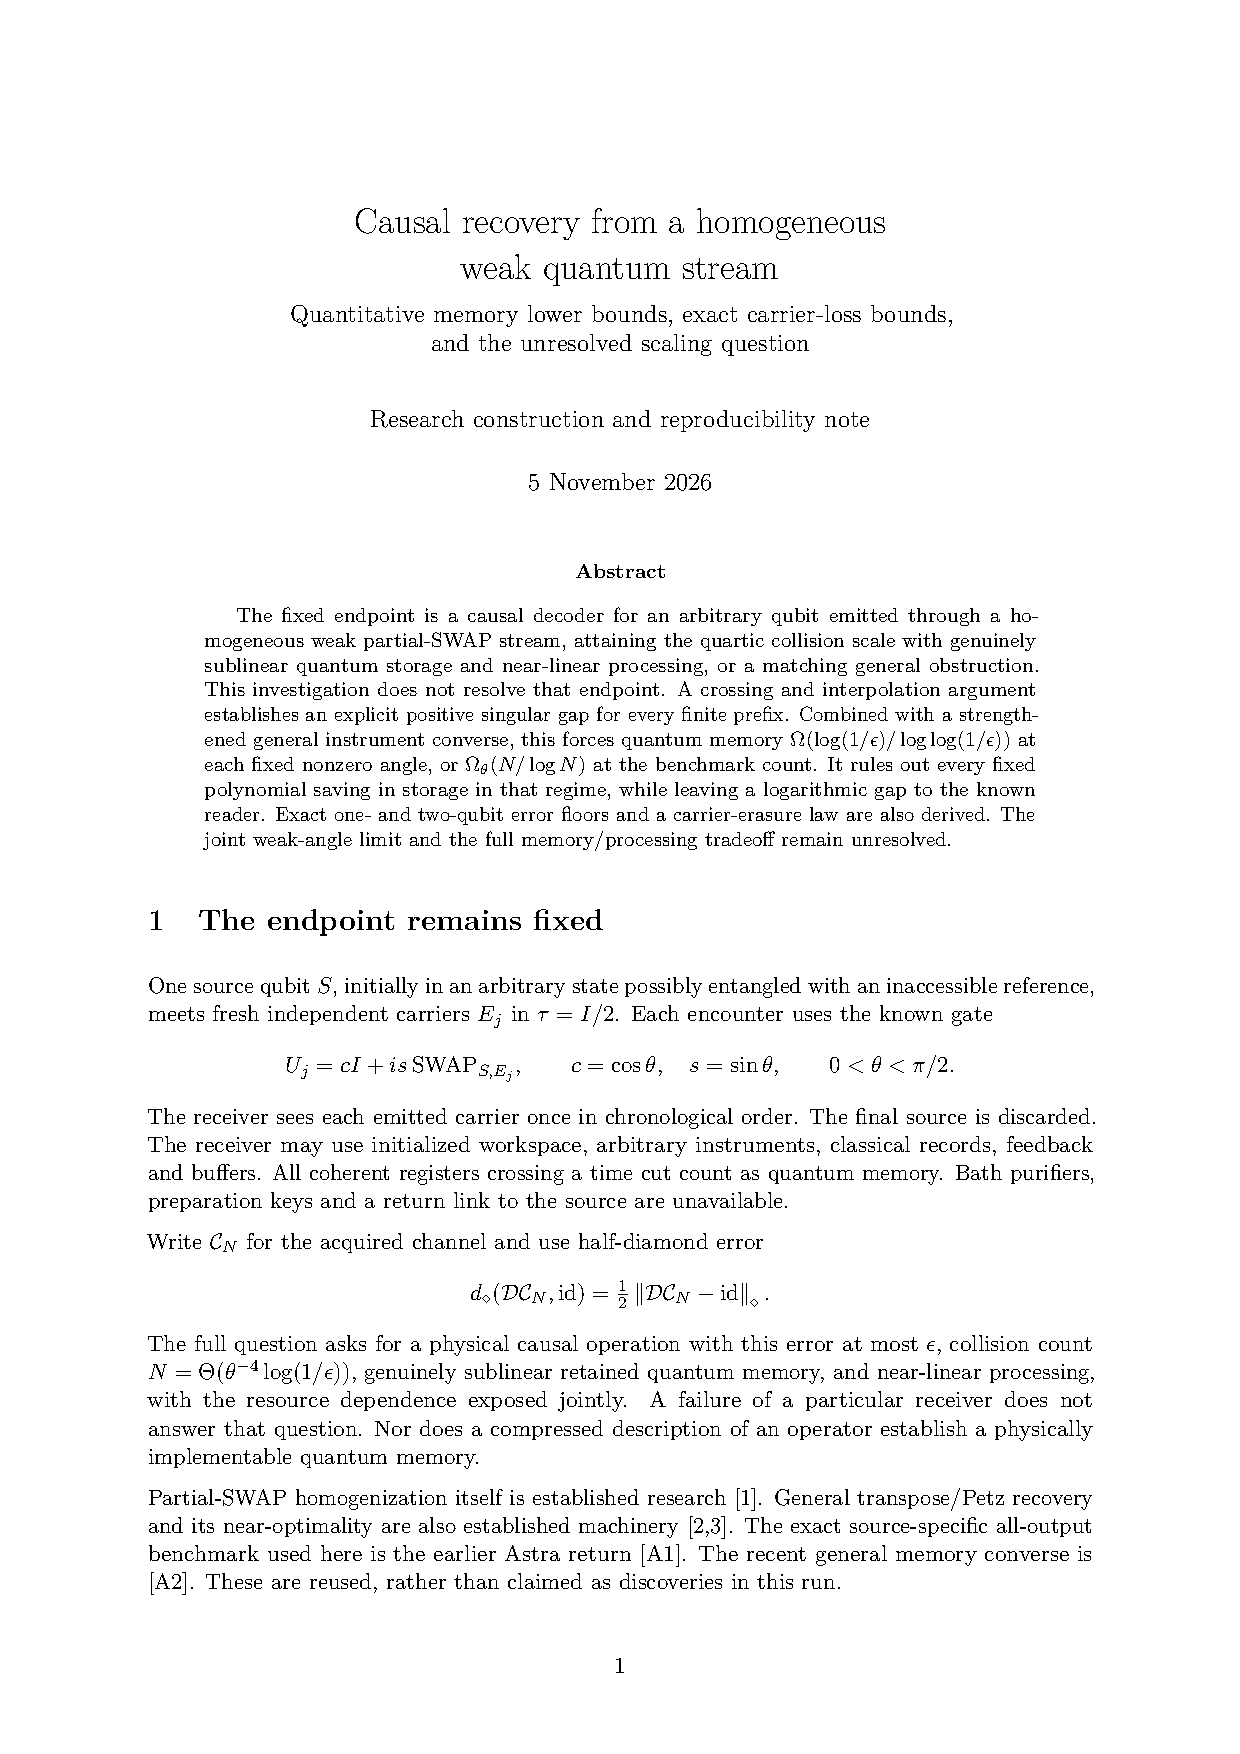
\includepdf[pages=-]{causal_recovery_research_note.pdf}
\end{document}
